

\section{Multiple Regression in R}

To illustrate multiple regression in R we'll use a built in dataset called |trees|. |trees| consists of measurements of the girth, height, and volume of 31 black cherry trees (|?trees| for more info). We'll start with some summary tables and diagnostic plots to familiarize ourselves with the data:
%
\begin{R}
> names(trees)
[1] "Girth"  "Height" "Volume"
> dim(trees)
[1] 31  3
> summary(trees)
     Girth           Height       Volume
 Min.   : 8.30   Min.   :63   Min.   :10.20
 1st Qu.:11.05   1st Qu.:72   1st Qu.:19.40
 Median :12.90   Median :76   Median :24.20
 Mean   :13.25   Mean   :76   Mean   :30.17
 3rd Qu.:15.25   3rd Qu.:80   3rd Qu.:37.30
 Max.   :20.60   Max.   :87   Max.   :77.00
> library(PerformanceAnalytics)
> chart.Correlation(trees)
\end{R}
%
As one might expect, the scatterplot matrix shows that all the variables are positively correlated, and girth and volume have a  particularly strong correlation.

Let's assume we're lumberjacks, but our permit only allows us to harvest a fixed number of trees.  We get paid by the total volume of wood we harvest, so we're interested in predicting a tree's volume (hard to measure directly) as a function of its girth and height (relatively easy to measure), so we can pick the best trees to harvest.  We'll therefore calculate a multiple regression of volume on height and width. Let's start by taking a look at the 3D scatter of the data using the plot3d function from the |rgl| package.
%
\begin{R}
> library(rgl)
> plot3d(trees, col='red', size=1, type='s') # use your mouse to rotate the plot
\end{R}
%
From the 3D scatter plot it looks like we ought to be able to find a plane through the data that fits the scatter fairly well. Let's use the |lm()| function to calculate the multiple regression:
%
\begin{R}
> l <- lm(Volume ~ Girth + Height, data=trees)
\end{R}
%
To visualize the multiple regression, let's use the |scatterplot3d| package to draw the 3D scatter of plots and the plane that corresponds to the regression model:
%
\begin{R}
> library(scatterplot3d)
> p <- scatterplot3d(trees,angle=55,type='h')
> title('Tree Volume as\na function of Girth and Height')
> p$plane3d(l, col='orangered')
> dev.copy(pdf, 'trees-regrfit.pdf')  # copy plot to a pdf file
> dev.off()  # write the file
\end{R}
%
Notice the use of |dev.copy()| and |dev.off()| to save the plot from the console.  The output this generates should look similar to Fig.~\ref{fig:treesregr}.
%
\begin{figure}[htbp]
\centering
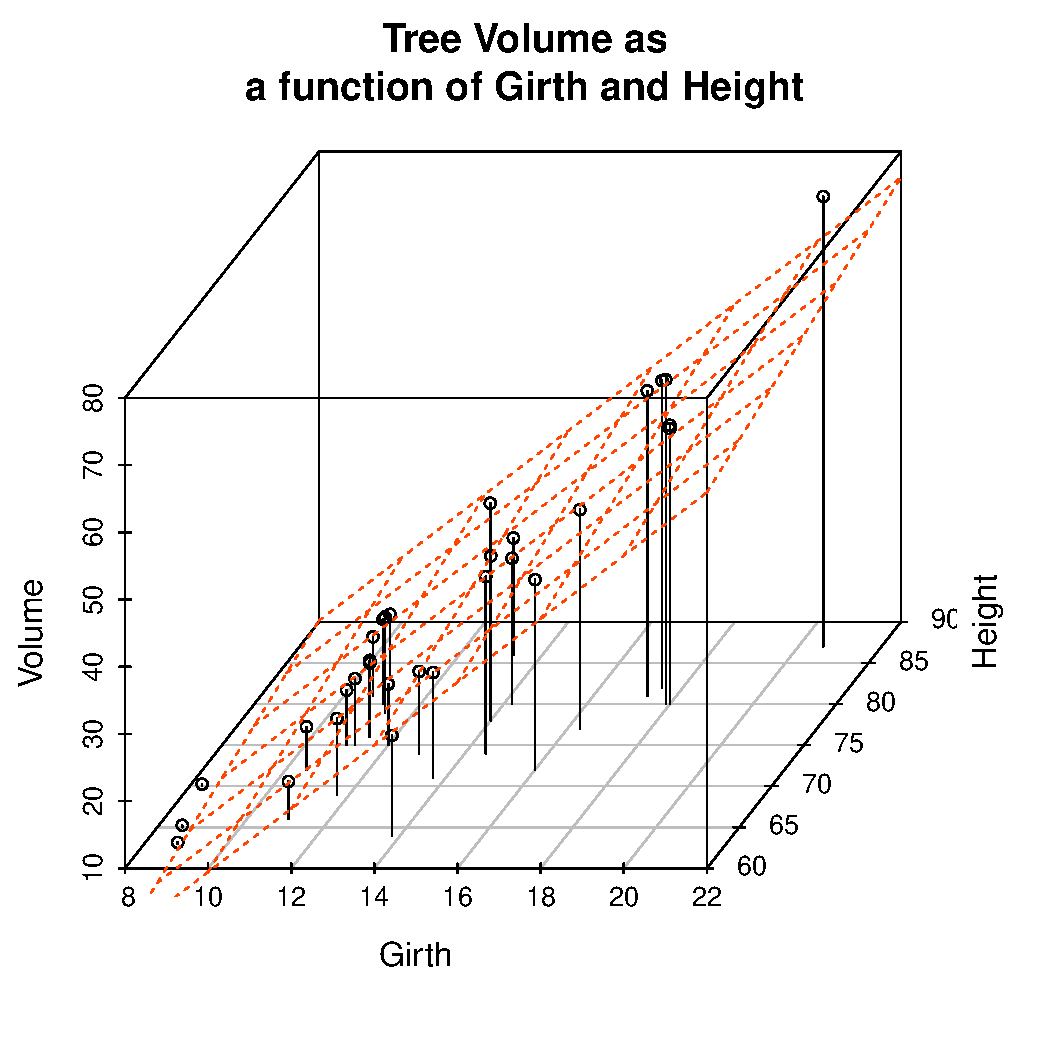
\includegraphics[width=0.5\columnwidth]{./figures/hands-on4/trees-regrfit.pdf}
\caption{Multiple regression plot of cherry tree volume on girth and height, generated using the \texttt{scatterplot3d} library\label{fig:treesregr}}
\end{figure}

From the figure it looks like the regression model fits pretty well, as we anticipated  from the pairwise relationships.  Let's use the |summary()| function to obtain details of the model:
\begin{R}
> summary(l)

Call:
lm(formula = Volume ~ Girth + Height, data = trees)

Residuals:
    Min      1Q  Median      3Q     Max
-6.4065 -2.6493 -0.2876  2.2003  8.4847

Coefficients:
            Estimate Std. Error t value Pr(>|t|)
(Intercept) -57.9877     8.6382  -6.713 2.75e-07 ***
Girth         4.7082     0.2643  17.816  < 2e-16 ***
Height        0.3393     0.1302   2.607   0.0145 *
---
Signif. codes:  0 ‘***’ 0.001 ‘**’ 0.01 ‘*’ 0.05 ‘.’ 0.1 ‘ ’ 1

Residual standard error: 3.882 on 28 degrees of freedom
Multiple R-squared: 0.948,  Adjusted R-squared: 0.9442
F-statistic:   255 on 2 and 28 DF,  p-value: < 2.2e-16
\end{R}
%
The regression equation is: $\hat{y} = 4.71x_1 + 0.34x_2$, where $y$ is Volume, and $x_1$ and $x_2$ are Girth and Height respectively. Since they're on different scales the coefficients for Girth and Height aren't directly comparable. Both coefficients are significant at the $p<0.05$ level, but that Girth is the much stronger predictor. In fact the addition of height explains only a minor additional fraction of variation in tree volume, so from the lumberjack's perspective the additional trouble of measuring height probably isn't worth it.

\subsection{Exploring the Vector Geometry of a Regression Model}

The object returned by the |lm()| function hold lots of useful information:
%
\begin{R}
> names(l)
 [1] "coefficients"  "residuals"     "effects"       "rank"          "fitted.values" "assign"
 [7] "qr"            "df.residual"   "xlevels"       "call"          "terms"         "model"
\end{R}
%
The |fitted.values| correspond to the predicted values of the outcome variable ($\hat{y}$). Let's use our knowledge of vector geometry to further explore the relationship between the predicted Volume and the predictor variables.  By definition the vector representing the predicted values lies in the plane defined by Height and Girth, so let's do some simple calculations to understand their length and angular relationships:
%
\begin{R}
# proportional to length of vectors
> sd(l$fitted.values)
[1] 16.00434
> sd(trees$Height)
[1] 6.371813
> sd(trees$Girth)
[1] 3.138139

# cosines of angles btw vectors
> cor(trees$Height, trees$Girth)
[1] 0.5192801
> cor(trees$Height, l$fitted.values)
[1] 0.6144545
> cor(trees$Girth, l$fitted.values)
[1] 0.9933158

# angles btw vectors in degrees
> acos(cor(trees$Height, l$fitted.values)) * (180/pi)
[1] 52.08771
> acos(cor(trees$Girth, l$fitted.values)) * (180/pi)
[1] 6.628322
> acos(cor(trees$Girth, trees$Height)) * (180/pi)
[1] 58.71603
\end{R}
%
Using those calculations above you should now be able to sketch out by hand, a diagram depicting the vector relationships between Height, Girth, and the predicted Volume.  Once you've finished with your sketch, discuss it with your fellow classmates.  Did you get similar answers? If not, discuss it and try to come up with an agreed upon representation.

\subsection{Exploring the Residuals from the Model Fit}

Now let's look at the residuals from the regression. The residuals represent the `unexplained' variance:
\begin{R}
> plot(trees$Volume,l$residuals, xlab='Volume',ylab='Regression Residuals')
> abline(h=0, lty='dashed', col='red')
\end{R}
%
Ideally the residuals should be evenly scatter around zero, with no trends as we go from high to low values of the outcome value.  As you can see in Fig.~\ref{fig:trees-resid} it looks like that the residuals on the left tend to be below zero, while those on the far right of the plot are consistently above zero, suggesting that there may be a non-linear aspect of the relationship that our model isn't capturing.
%
\begin{figure}[htbp]
\centering
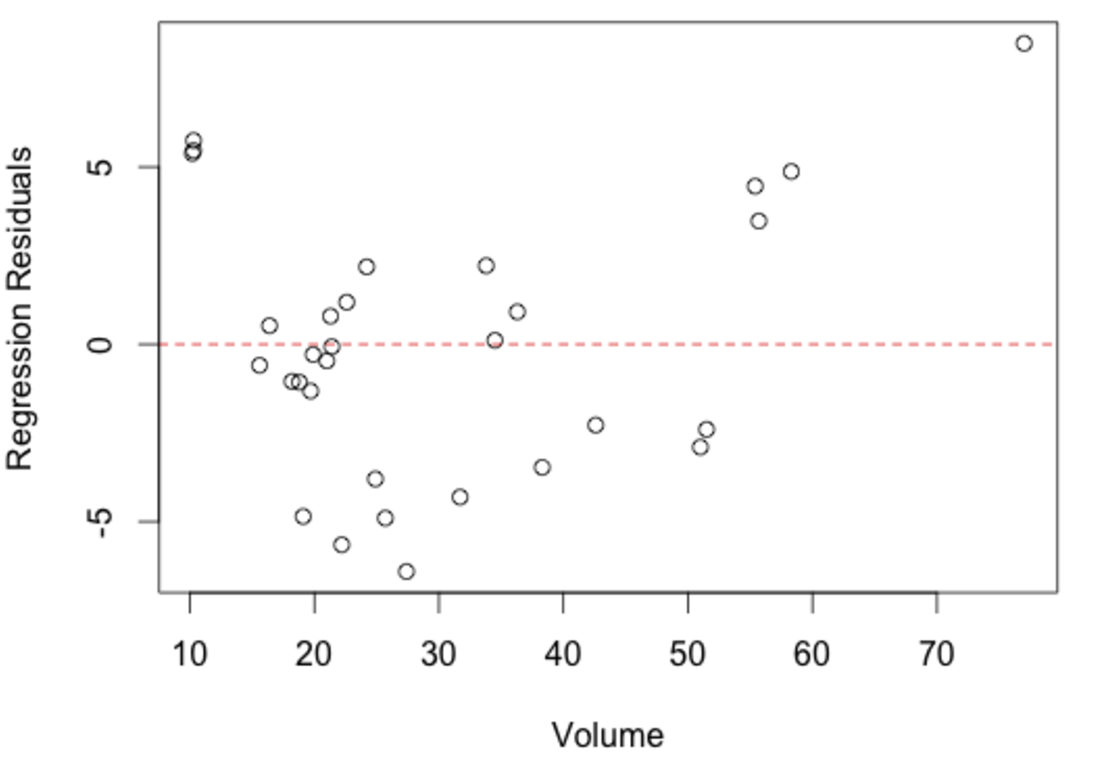
\includegraphics[height=1.5in]{./figures/hands-on4/trees-residuals.pdf}
\caption{Residual plot based on the multiple regression plot of cherry tree volume on girth and height,\label{fig:trees-resid}}
\end{figure}

Let's think about the relationships we're actually modeling for a few minutes.  For the sake of simplicity let's consider the trunk of a tree to be a cylinder.  How do the dimensions of this cylinder relate to it's volume? You can look up the formula for the volume of a cylinder, but the key thing you'll want to note is that volume of the cylinder should be proportional to a characteristic  length of the cylinder  ($V \propto \mathrm{L}^3$). This suggests that if we want to fit a linear model we should relate Girth to $\sqrt[3]{\mathrm{Volume}}$. Let's explore this a little. Since our initial multiple regression suggested that height had relatively little predictive power, we'll simplify our model down to a single predictor:
%
\begin{R}
> cuberoot.V <- trees$Volume^0.33
> cor(trees$Volume, trees$Girth)
[1] 0.9671194
> cor(cuberoot.V, trees$Girth)
[1] 0.9777078
> l.orig <- lm(trees$Volume~ trees$Girth)
> l.transf <- lm(cuberoot.V ~ trees$Girth)
> summary(l.orig)

Call:
lm(formula = trees$Volume ~ trees$Girth)

Residuals:
   Min     1Q Median     3Q    Max
-8.065 -3.107  0.152  3.495  9.587

Coefficients:
            Estimate Std. Error t value Pr(>|t|)
(Intercept) -36.9435     3.3651  -10.98 7.62e-12 ***
trees$Girth   5.0659     0.2474   20.48  < 2e-16 ***
---
Signif. codes:  0 ‘***’ 0.001 ‘**’ 0.01 ‘*’ 0.05 ‘.’ 0.1 ‘ ’ 1

Residual standard error: 4.252 on 29 degrees of freedom
Multiple R-squared: 0.9353, Adjusted R-squared: 0.9331
F-statistic: 419.4 on 1 and 29 DF,  p-value: < 2.2e-16

> summary(l.transf)

Call:
lm(formula = cuberoot.V ~ trees$Girth)

Residuals:
     Min       1Q   Median       3Q      Max
-0.18919 -0.09775 -0.01488  0.07855  0.26427

Coefficients:
            Estimate Std. Error t value Pr(>|t|)
(Intercept)  0.82543    0.08856   9.321 3.18e-10 ***
trees$Girth  0.16324    0.00651  25.076  < 2e-16 ***
---
Signif. codes:  0 ‘***’ 0.001 ‘**’ 0.01 ‘*’ 0.05 ‘.’ 0.1 ‘ ’ 1

Residual standard error: 0.1119 on 29 degrees of freedom
Multiple R-squared: 0.9559, Adjusted R-squared: 0.9544
F-statistic: 628.8 on 1 and 29 DF,  p-value: < 2.2e-16
\end{R}
%
Comparing the summary tables, we see indeed that using the cube root of Volume improves the fit of our model some. Let's examine the residuals.
%
\begin{R}
> layout(c(1,2), widths=c(3,3), heights=c(2,2))
> plot(trees$Volume, l.orig$residuals, xlab='Volume', ylab="Residuals")
> abline(h = 0, col='red', lty='dashed')
> plot(cuberoot.V, l.transf$residuals, xlab='Volume^0.33', ylab='Residuals')
> abline(h = 0, col='red', lty='dashed')
> dev.copy(pdf, 'compare-residuals.pdf')
> dev.off()
\end{R}
%
\begin{figure}[htbp]
\centering
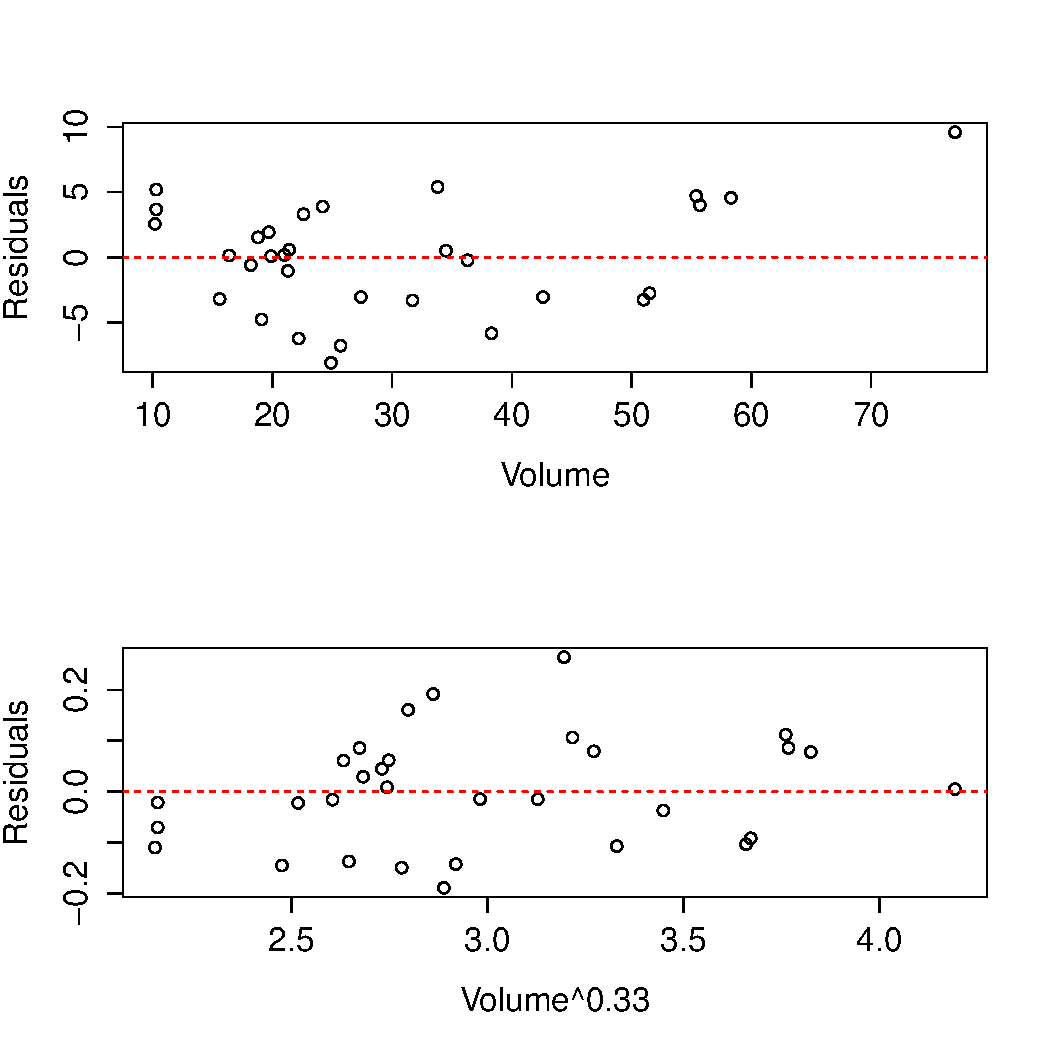
\includegraphics[height=2in]{./figures/hands-on4/compare-residuals.pdf}
\caption{Residual plot based on the bivariate regression of tree volume on girth, or $\sqrt[3]{V}$ on girth \label{fig:compare-resid}}
\end{figure}
%
As we can see the transformation we applied to the data did seem to make our residuals more uniform across the range of observations. Note the use of the |layout()| function to put multiple plots in the same figure.

Above we transformed the volume data in order to fit a straight line relationship between $\sqrt[3]{V}$  and Girth. However, we could just as easily have applied a cubic regression to the original variables as shown below (remember this is still linear regression in the coefficients):

\begin{R}
> lm.3 <- lm(Volume ~ I(Girth^3), data=trees)
> summary(lm.3)

Call:
lm(formula = Volume ~ I(Girth^3), data = trees)

Residuals:
   Min     1Q Median     3Q    Max
-4.526 -3.036  0.215  2.419  8.291

Coefficients:
             Estimate Std. Error t value Pr(>|t|)
(Intercept) 8.0426960  1.0426698   7.714 1.66e-08 ***
I(Girth^3)  0.0081365  0.0003118  26.098  < 2e-16 ***
---
Signif. codes:  0 ‘***’ 0.001 ‘**’ 0.01 ‘*’ 0.05 ‘.’ 0.1 ‘ ’ 1

Residual standard error: 3.379 on 29 degrees of freedom
Multiple R-squared: 0.9592, Adjusted R-squared: 0.9578
F-statistic: 681.1 on 1 and 29 DF,  p-value: < 2.2e-16

> lm.3$coefficients
(Intercept)  I(Girth^3)
8.042696007 0.008136533
> a0 = lm.3$coefficients[[1]]
> B1 = lm.3$coefficients[[2]]
> x <- seq(8,20,0.25) # range of values to evaluate model over
> fit <- a0 + B1*x^3
> plot(Volume ~ Girth, data=trees)
> lines(x,fit,col='red')
> figtext <- paste(c("Volume = ", round(a0,2), "+", round(B1,4), "*Girth^3"),collapse='')
> text(12, 60, figtext)
\end{R}
%
\begin{figure}[htbp]
\centering
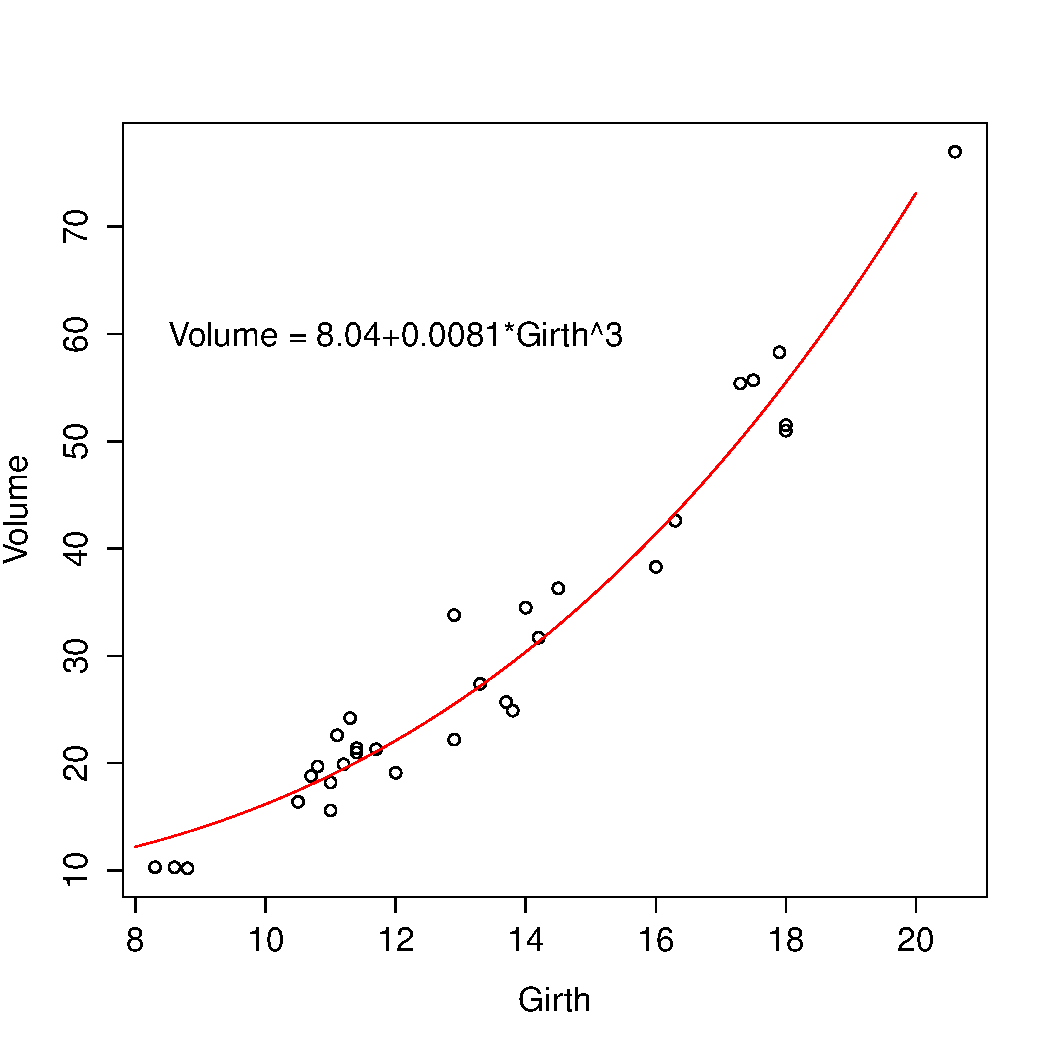
\includegraphics[height=2in]{./figures/hands-on4/cubic-regr.pdf}
\caption{Cubic regression of tree volume on girth \label{fig:cubic-regr}}
\end{figure}
%


\medskip
\begin{assignment}
In the same R markdown docoument you created for Assignment 4.1, write a function, |mult.regr(X,y)| that calculates the multiple regression of $y$ on multiple predictors, $x_1, x_2, \ldots x_k$ \emph{using matrix operations}. Your function should take two arguments, |X| and |y|, where |X| is a matrix representing the predictor variables and |y| is a vector for the outcome variable.  Your function should return a list containg the vector of regression coeffients, $B$, the coefficient of determination ($R^2$), and a vector, $\hat{y}$, representing the fitted values.  Refer to the slides from lecture 4 (and possibly lecture 2 if you need a refresher) to review the matrix  solution to the regression problem.
\end{assignment}